\documentclass[letterpaper, french]{article}
\usepackage{aaai18}
\usepackage{times}
\usepackage{helvet}
\usepackage{courier}
\usepackage{url}
\usepackage{graphicx}

\usepackage{tikz}
\usepackage{pgfplots}
\pgfplotsset{compat=1.14}

\frenchspacing 
% Add additional packages here. The following 
% packages may NOT be used (this list 
% is not exhaustive): 
% authblk, caption, CJK, float, fullpage, geometry, 
%hyperref, layout, nameref, natbib, savetrees, 
%setspace, titlesec, tocbibind, ulem
\usepackage{amsmath}
\usepackage{amsfonts}
\usepackage{amssymb}
\usepackage[french]{babel}
\selectlanguage{french}
\usepackage[T1]{fontenc}
\usepackage[utf8]{inputenc}
%US Lettersize Paper Is Required 
\setlength{\pdfpagewidth}{8.5in}
\setlength{\pdfpageheight}{11in}
% 
% 
% PDFINFO 
% You are required to complete the following 
% for pass-through to the PDF. 
% No LaTeX commands of any kind may be 
% entered. The parentheses and spaces 
% are an integral part of the 
% pdfinfo script and must not be removed. 
% 
\pdfinfo{ 
/Title (DDPG : explication de l'algorithme et analyse expérimentale sous différentes contraintes) 
/Author (Quentin Lenet, Justine Pepin, Arnaud Venet) 
} 
% 
%Section Numbers 
% Uncomment if you want to use section numbers 
% and change the 0 to a 1 or 2 
% 
\setcounter{secnumdepth}{0}
% Title and Author Information Must Immediately Follow 
% the pdfinfo within the preamble 
% 
\title{DDPG : explication de l'algorithme et analyse expérimentale sous différentes contraintes} 
\author {Quentin \textsc{Lenet}, Justine \textsc{Pepin}, Arnaud \textsc{Venet} \\
École Polytechnique de Montréal }
%
% 
\begin{document} 
\maketitle 
\begin{abstract} 
L'algorithme \textit{Deep Deterministic Policy Gradient} (DDPG) présenté dans l'article étudié \cite{ddpg} est une méthode d'apprentissage par renforcement profond pouvant apprendre des politiques dans un espace d'actions continu. L'implémentation de cet algorithme nécessite l'utilisation de nombreux hyperparamètres. Nous avons donc voulu déterminer la robustesse de l'algorithme vis-à-vis des réglages expérimentaux différents de ceux proposé dans l'article. Nos résultats montrent que le type de bruit importe peu, ce qui compte est d'en avoir en quantité raisonnable. De même, pour les légères modifications de l'architecture du réseau, les résultats sont très similaires.
% Ce qu'est DDPG en gros et qu'est-ce 
% qu'on va faire avec et qu'étaient grossièrement 
% les résultats

\end{abstract} 


\section{Introduction}
Cette première section portera sur les travaux antérieurs à DDPG dans la littérature. Il y en a deux qui sont spécialement importants puisqu'ils sont les prédécesseurs de DDPG; ils seront détaillés dans les prochains paragraphes.
% Introduire les travaux précédents dans la littérature
% Comme on faisait dans notre super présentation
\subsection{DQN - Première influence de DDPG}
\paragraph{}
DQN (\textit{Deep Reinforcement Learning}) utilise un réseau de neurones pour apprendre à un agent une politique. Il a été présenté par DeepMind technologies en 2013 \cite{mnih2013playing}. Cet algorithme peut apprendre une politique à un agent qui évolue dans un environnement avec un espace d'états très grand. En effet, le réseau de neurones joue le rôle de la fonction $\mathcal{Q}$ qui prend à sa couche d'entrée les états, et retourne en sortie, à l'aide d'un softmax, quelle action discrète emprunter. Plusieurs améliorations ont été proposées pour cet algorithme, comme le \textit{replay buffer} (mémoire de reprise). Celui-ci emmagasine les transitions d'un état à un autre rencontrées lors de l'apprentissage. Une transition se présente sous cette forme $(s_t, a_t, r_t, s_{t+1})$ pour un agent qui passe de l'état $s_t$ à l'état $s_{t+1}$ en ayant effectué l'action $a_t$ et qui a reçu la récompense $r_t$. La mémoire de reprise, en enregistrant beaucoup de transitions, peut retourner des lots aléatoires composés de plusieurs transitions non successives. Ceci apporte de la stabilité à l'algorithme lors de l'apprentissage. Une autre amélioration proposée par Van Hasselt et al. est l'ajout d'un \textit{target network} (réseau cible) $\mathcal{Q\prime}$, \cite{wang2015dueling} \cite{wang2015dueling}. Ce réseau cible est initialisé avec les mêmes poids que le réseau initial, et sa mise à jour est faite à partir de ce dernier, avec la formule de Polyak.
\begingroup
\begin{center}
\begin{equation}\label{eq:q_update}
\begin{split}
 Q\prime = (1-\tau) Q\prime + \tau Q
\end{split}
\end{equation}
\end{center}
\endgroup
Après l'initialisation, pour le reste de l'apprentissage, le paramètre $\tau$ est pris petit (vers 0.01), pour adoucir la mise à jour du réseau cible. Ceci ajoute encore de la stabilité à l'apprentissage.
\paragraph{}
Cet algorithme présente certaines limites et ne peut pas s'appliquer aux environnements trop complexes. Les choix d'actions sélectionnables par l'agent restent restreints; pour évoluer d'un état à l'autre, notre agent n'a le choix qu'entre quelques actions dont le nombre correspondra au nombre de neurones de la couche de sortie. Pour que l'agent puisse effectuer un grand nombre d'actions, voire des actions continues, il faut aller voir d'autres approches et d'autres algorithmes.

\subsection{DPG - Deuxième influence de DDPG}
DPG (\textit{Deterministic Policy Gradient}) est un algorithme qui a été présenté en 2014 par des gens de chez DeepMind \cite{silver2014deterministic}. Il vise à éviter les intégrales trop laborieuses à calculer en utilisant le gradient d'une politique déterministe au lieu de celui d'une politique stochastique. Ainsi, on peut améliorer la performance et l'efficacité dans l'estimation du gradient par rapport au Q-learning, qui, lorsqu'appliqué directement aux espaces d'actions continus, tente d'optimiser l'action $a$ au temps $t$ à chaque pas de temps pour trouver la politique optimale, ce qui est bien sûr vorace en temps lorsqu'on se sert d'un grand espace d'actions.\\

DPG est un algorithme avec un acteur et un critique où typiquement l'acteur ajuste les paramètres en performant la descente des gradients, tandis que le critique estime la fonction d'utilité selon l'action. Dans notre cas, le critique utilise tout comme dans DQN l'équation de Bellman, mais comme DPG travaille avec une politique déterministe, la fonction représentant la politique du choix d'action $\mu (s|\theta^\mu)$ associe directement chaque état $s$ avec une action $a$, ce qui fait qu'on peut éviter l'espérance qui se trouve normalement en milieu d'équation.
\begingroup
\begin{center}
\begin{equation}\label{eq:critiqueAvecDeterministe}
\begin{split}
 Q^{\mu}(s_t, a_t) = \mathbb{E}_{r_t, s_{t+1}\sim E} \left[r(s_t, a_t)+ \gamma Q^{\mu}(s_{t+1}, \mu(s_{t+1}))\right]
\end{split}
\end{equation}
\end{center}
\endgroup
On utilise l'erreur quadratique pour la fonction de perte, \textit{MSELoss}, pour mettre à jour notre $\mathcal{Q}$.
\begingroup
\begin{center}
\begin{equation}\label{eq:perte}
\begin{split}
L = \frac{1}{N} \Sigma_i (y_i - \mathcal{Q}(s_i, a_i|\theta^{\mathcal{Q}}))^2
\end{split}
\end{equation}
\end{center}
\endgroup
Du côté de l'acteur, pour apprendre la politique déterministe cible ${\mu}_{\theta (s)}$, on utilise des trajectoires générées par une politique stochastique arbitraire $\pi (s, a)$. Avec celle-ci, on peut calculer le gradient de la performance $J$.
\begingroup
\begin{center}
\begin{equation}\label{eq:acteur}
\begin{split}
 \triangledown_{\theta^{\mu}}J \approx \mathbb{E}_{s_t \sim \rho^\beta} \left[\triangledown_{a}\mathcal{Q}(s, a|\theta^{\mathcal{Q}})|_{s=s_t, a=\mu(s_t)}\triangledown_{\theta_{\mu}}\mu(s|\theta^{\mu})|_{s=s_t}\right]
\end{split}
\end{equation}
\end{center}
\endgroup
Un détail intéressant à propos du gradient de la politique déterministe est qu'il s'agit d'un cas limite de la politique stochastique; c'est pourquoi on peut employer la version déterministe au même titre que celle stochastique, avec bien entendu des façons de faire différentes et des avantages différents. Justement, un avantage potentiel d'utiliser une politique déterministe est de contourner l'échantillonnage d'importance, qui utilise les retours de la politique d'apprentissage $\pi (s, a)$ et qui permet de les ajuster à la politique de notre choix. Typiquement, pour les algorithmes de type acteur-critique comme le nôtre, mais qui font le choix d'action glouton avec une politique stochastique, on doit faire l'échantillonnage d'importance pour l'acteur comme pour le critique. Toutefois, DPG tire bien son épingle du jeu et permet d'éviter la très grande variance qui peut survenir avec l'échantillonnage d'importance grâce à la disparition d'une intégrale dans les calculs pour l'acteur lorsqu'on change la politique stochastique en politique déterministe. Finalement, on peut l'éviter aussi une seconde fois dans le critique en utilisant le Q-learning.

\section{Approche théorétique}
% Ce qui distingue DDPG
% Comparer avec A-C
% Comparer avec TRPO
\subsection{DDPG plus en détail}
DDPG (\textit{Deep Deterministic Policy Gradient}) s'inscrit à la fois dans la lignée de DPG et dans la lignée de DQN puisqu'il reprend volontiers les points caractéristiques de ces deux algorithmes et les intègre ensemble pour former un algorithme hybride. Les points repris sont notamment : l'usage d'un tampon pour rejouer les séquences d'apprentissage, la mémoire de reprise, ce qui permet de mettre à jour les paramètres du réseau à partir d'échantillons distribués indépendamment et équitablement; la mise à jour adoucie des poids d'un réseau cible, ce qui permet d'avoir une plus grande stabilité dans l'apprentissage; ainsi qu'un modèle d'algorithme acteur-critique avec le choix d'action glouton et une politique déterministe. \\

Également, quelques techniques supplémentaires ont été utilisées pour obtenir un meilleur apprentissage, comme la normalisation des lots \cite{batch-norm}, qui permet d'éviter les entrées trop disparates qui augmentent la difficulté que les réseaux ont à trouver les bons hyperparamètres, ou encore comme l'ajout de bruit pour explorer plus efficacement l'espace d'action continu. Pour ce faire, on peut tout simplement ajouter $\mathcal{N}$ à notre politique, où $\mathcal{N}$ peut être n'importe quel type de bruit qui convient à notre environnement.
\begingroup
\begin{center}
\begin{equation}\label{eq:bruit}
\begin{split}
\mu\prime(s_t) = \mu(s_t|\theta_{t}^{\mu}) + \mathcal{N}
\end{split}
\end{equation}
\end{center}
\endgroup
Dans l'article de DDPG, le bruit proposé était généré par le processus d'Ornstein-Uhlenbeck \cite{ornstein-uhlenbeck}. Ce processus simule un mouvement brownien avec friction d'une particule. Il existe alors une autocorrélation temporelle du bruit. \\

%(perfomance du truc) et dire ce qu'on va tenter de faire avec??
En somme, décrit grossièrement, DDPG est un algorithme qui combine DQN et DPG. Il doit donc entretenir quatre réseaux de neurones : un acteur, un critique, un acteur cible et un critique cible. Les figures \ref{fig:reseau_acteur} et \ref{fig:reseau_critique} montrent de façon visuelle à quoi ressemblent ces réseaux. Les réseaux cible subissent des mises à jour adoucies à partir de leur réseau d'apprentissage respectif, et ces derniers s'entraînent à partir de mémoires de reprise. Il y a également de la normalisation de lots pour optimiser l'apprentissage et du bruit pour prévenir le surapprentissage. Tout cet ensemble permet d'obtenir un algorithme à performance satisfaisante sur les environnements qui ont de grands espaces d'actions et d'états.

\begin{figure}
\begin{center}

\def\layersep{2.5cm}

\begin{tikzpicture}[shorten >=1pt,->,draw=black!50, node distance=\layersep, scale = 1]
    \tikzstyle{every pin edge}=[<-,shorten <=1pt]
    \tikzstyle{neuron}=[circle,fill=black!25,minimum size=25pt,inner sep=0pt]
    \tikzstyle{input neuron}=[neuron, fill=green!20, draw=green];
    \tikzstyle{output neuron}=[neuron, fill=red!20, draw=red];
    \tikzstyle{hidden neuron}=[neuron, fill=blue!20, draw=blue];
    \tikzstyle{annot} = [text width=4em, text centered]

    % Draw the input layer nodes
    \foreach \name / \y in {1,...,4}
    % This is the same as writing \foreach \name / \y in {1/1,2/2,3/3,4/4}
        \node[input neuron] (I-\name) at (0,-1-\y) {$S_{\name}$};


    % Draw the hidden layer nodes
    % H1
    \foreach \name / \y in {1,...,5}
        \node[hidden neuron] (H1-\name) at (\layersep,-\y) {$\name$};
    \path[yshift=-0.3cm]
    		node[hidden neuron] (H1-6) at (\layersep,-6) {$400$};
    		
    	% H2
    \foreach \name / \y in {1,...,5}
        \node[hidden neuron] (H2-\name) at (2*\layersep,-\y) {$\name$};
    \path[yshift=-0.3cm]
    		node[hidden neuron] (H2-6) at (2*\layersep,-6) {$300$};

    		

    % Draw the output layer node
    \foreach \name / \y in {1,...,2}
     	\node[output neuron] (O-\name) at (3*\layersep,-2-\y) {$A_{\name}$};


	% ...
	\foreach \ID in {H1,H2}
		\path (\ID-5) edge[-,densely dotted] (\ID-6);

	
	% Connect layers
	\foreach \source in {1,...,4}
	{
        \foreach \dest in {1,...,6}
        {
        		% input layer to first hidden layer
        		\path (I-\source) edge (H1-\dest); 
		}
			  	
	}
	\foreach \source in {1,...,6}
	{
		\foreach \dest in {1,...,6}
        {
			% hidden layers
			\path (H1-\source) edge (H2-\dest);
		}
		\foreach \dest in {1,...,2}{
			% hidden layer 2 to output
            \path (H2-\source) edge (O-\dest);
		}
	}
            

    % Annotate the layers
    \node[annot,above of=H1-1, node distance=1cm] (h1) {Couche cachée $1$};
    \node[annot,above of=H2-1, node distance=1cm] (h2) {Couche cachée $2$};
    \node[annot,left of=h1] {Paramètres d'état};
    \node[annot,right of=h2] {Paramètres d'action};
\end{tikzpicture} 
\caption{Réseau acteur $\mu$}
\label{fig:reseau_acteur}
\end{center}
\end{figure}

\begin{figure}
\begin{center}


\def\layersep{2.5cm}

\begin{tikzpicture}[shorten >=1pt,->,draw=black!50, node distance=\layersep, scale = 1]
    \tikzstyle{every pin edge}=[<-,shorten <=1pt]
    \tikzstyle{neuron}=[circle,fill=black!25,minimum size=25pt,inner sep=0pt]
    \tikzstyle{input neuron}=[neuron, fill=green!20, draw=green];
    \tikzstyle{output neuron}=[neuron, fill=red!20, draw=red];
    \tikzstyle{hidden neuron}=[neuron, fill=blue!20, draw=blue];
    \tikzstyle{annot} = [text width=4em, text centered]

    % Draw the input layer nodes
    \foreach \name / \y in {1,...,4}
    % This is the same as writing \foreach \name / \y in {1/1,2/2,3/3,4/4}
        \node[input neuron] (I-\name) at (0,-1-\y) {$S_{\name}$};


    % Draw the hidden layer nodes
    % H1
    \foreach \name / \y in {1,...,5}
        \node[hidden neuron] (H1-\name) at (\layersep,-\y) {$\name$};
   
    \path[yshift=-0.3cm]
    	node[hidden neuron] (H1-6) at (\layersep,-6) {$400$};
   	
    	
    	\foreach \name / \y in {1,...,2}
     	\node[output neuron] (A-\name) at (\layersep,-6.5-\y) {$A_{\name}$};
   		
    	% H2
    \foreach \name / \y in {1,...,5}
        \node[hidden neuron] (H2-\name) at (2*\layersep,-\y) {$\name$};
    \path[yshift=-0.3cm]
    		node[hidden neuron] (H2-6) at (2*\layersep,-6) {$300$};

    		

    % Draw the output layer node
     \node[output neuron] (O) at (3*\layersep,-3) {$\mathcal{Q}$};


	% ...
	\foreach \ID in {H1,H2}
		\path (\ID-5) edge[-,densely dotted] (\ID-6);

	
	% Connect layers
	\foreach \source in {1,...,4}
	{
        \foreach \dest in {1,...,6}
        {
        		% input layer to first hidden layer
        		\path (I-\source) edge (H1-\dest); 
		}	  	
	}
	\foreach \source in {1,...,6}
	{
		\foreach \dest in {1,...,6}
        {
			% hidden layers
			\path (H1-\source) edge (H2-\dest);
		}
	}
	
	\foreach \source in {1,...,2}
	{
		\foreach \dest in {1,...,6}
        {
			% hidden layers
			\path (A-\source) edge (H2-\dest);
		}
	}
	
	
	% hidden layer 2 to output
	\foreach \source in {1,...,6}{
        \path (H2-\source) edge (O);
	}	
            
            
                        

    % Annotate the layers
    \node[annot,above of=H1-1, node distance=1cm] (h1) {Couche cachée $1$};
    \node[annot,above of=H2-1, node distance=1cm] (h2) {Couche cachée $2$};
    \node[annot,left of=h1] {Paramètres d'état};
    \node[annot,right of=h2] {Sortie};
\end{tikzpicture} 
\caption{Réseau critique $\mathcal{Q}$}
\label{fig:reseau_critique}
\end{center}
\end{figure}

\subsection{DDPG et les modèles classiques d'Acteur-Critique}
Les méthodes dites d'acteur-critique implémentent de façon générale l'itération de la politique en alternant entre une étape d'évaluation de la politique et une étape d'amélioration de la politique \cite{LectureActor-critic}. Le critique est en charge d'évaluer la politique dans son état présent, tandis que l'acteur est en charge de l'améliorer s'il réussit à trouver une action qui est meilleure que celle recommandée par la politique présente. Dans le cas où l'espace des actions et l'espace des états sont très grands, l'acteur comme le critique utilisent des approximateurs compatibles de fonctions, ces dernières étant trop complexes pour être évaluées directement. Comme l'acteur utilise une Q-valeur pour la mise à jour de la politique, le critique doit estimer la Q-fonction. Pour les grands espaces d'états, la différence temporelle des moindres carrés peut servir à estimer la Q-fonction. Quant à l'acteur, il performe d'ordinaire la descente de gradient stochastique sur la surface générée par les performances de la politique. \\

Il y a donc quelques différences entre DDPG et la version plus classique d'un acteur-critique, qui proviennent de DQN comme de DPG. Par exemple, DQN amène la notion de réseau cible qui ne se trouve pas dans le modèle acteur-critique de base, ou encore DPG amène la notion de politique de gradient déterministe alors que les algorithmes acteur-critique jusque-là se servaient de la politique de gradient stochastique. Néanmoins, DDPG reste, de par sa logique qui distingue le rôle d'acteur du rôle de critique de la même façon que le font les modèles classiques d'acteur-critique, dans la lignée de ce type d'algorithme.\\

Il faudrait aussi souligner que les méthodes utilisant des politiques déterministes comme DDPG ne sont pas la manne des algorithmes. D'autres algorithmes qui optimisent des politiques stochastiques de contrôle sont très efficaces sur les environnements dotés de grands espaces d'actions et d'états, comme par exemple TRPO (\textit{Trust Region Policy Optimization}) \cite{TRPO}, qui fait lui aussi plusieurs itérations afin de corriger graduellement une politique. Pour faire son approximation du retour de la politique, TRPO utilise une pénalité de divergence KL (\textit{Kullback-Leibler}) qui est une méthode assez différente que ce qui est fait avec DDPG. Toutefois, un bon avantage de DDPG vis-à-vis de TRPO reste sa vitesse, puisqu'il est très facile de manipuler les politiques déterministes comparativement à celles stochastiques.

\section{Résultats des expériences et discussion}
Nous avons implémenté DDPG en suivant les algorithmes présentés dans l'article. L'environnement utilisé pour les tests est OpenAI Gym, qui intègre quelques problèmes à la physique réaliste mais simplifiés du moteur MuJoCo \cite{MuJoCo}. Ceux-ci consistent généralement à contrôler différentes articulations d'un modèle caricatural d'animal ou d'humanoïde pour effectuer une séquence de gestes précis.
\smallbreak
Intrigués par certains choix d'hyperparamètres qui n'étaient pas très bien justifiés dans l'article de DDPG, nous avons décidé de modifier le bruit d'exploration afin de voir en quoi il permet d'améliorer la convergence de l'apprentissage. Dans un premier temps, considérons un bruit d'exploration unifome (variance plus grande par rapport à un processus gaussien).\\
Commençons par un problème simple : pendulum, qui consiste à actionner une liaison pivot pour placer une tige à la verticale, en équilibre au dessus de la liaison.

\begin{figure}[!h]
\begin{center}
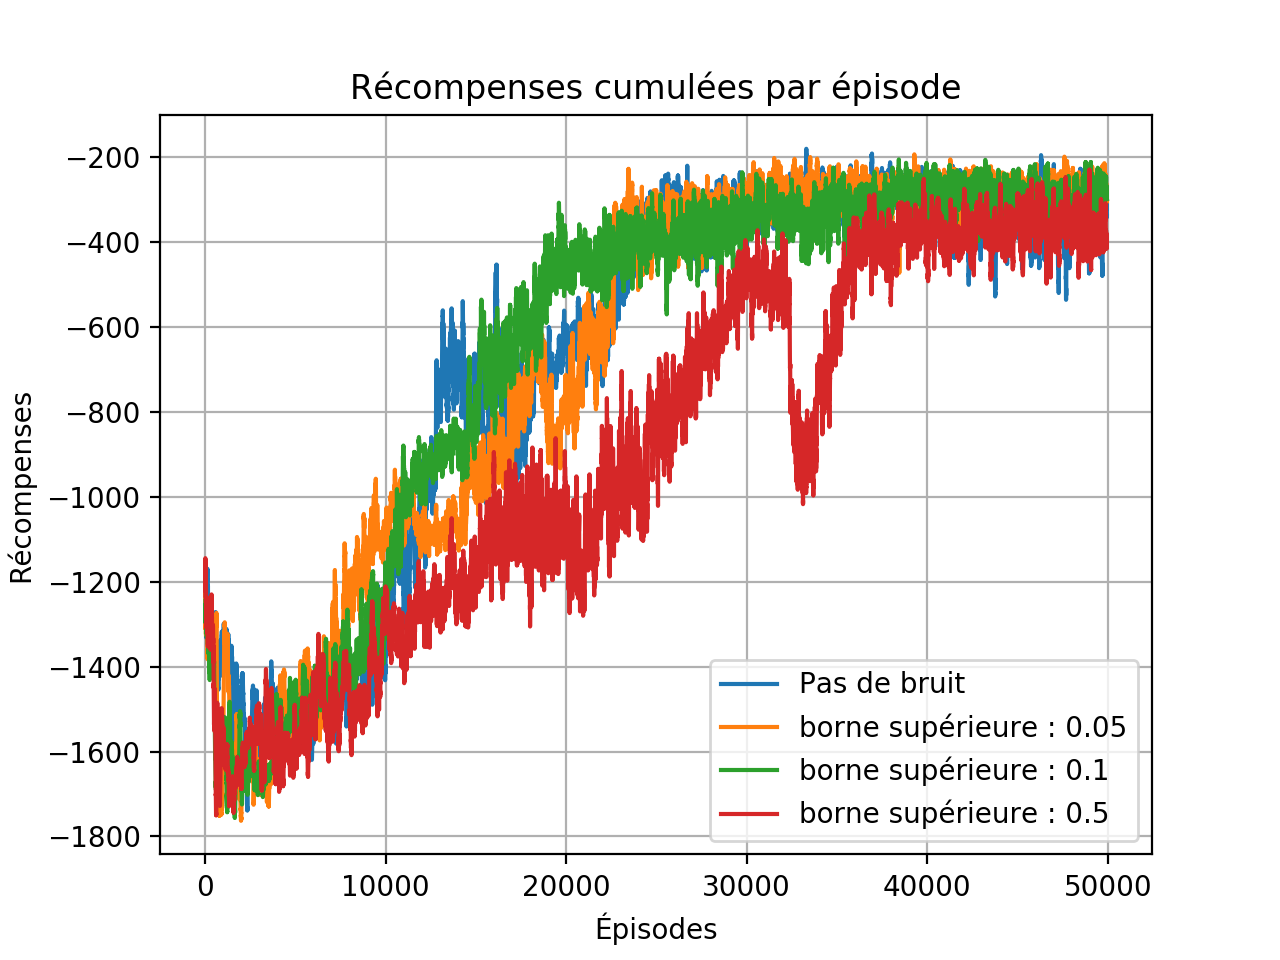
\includegraphics[scale=0.5]{assiettes/pendulum_uniform.png}
\caption{Influence d'un bruit uniforme centré pour le pendule}
\label{fig3}
\end{center}
\end{figure}
Nous voyons sur la figure~\ref{fig3} qu'à part le cas où un très grand bruit d'exploration (entre -0.5 et +0.5, sachant que les actions sont bornées entre -1 et +1) est imposé, les performances sont peu impactées par le choix du bruit.
\smallbreak
Poursuivons avec un problème plus complexe, nommé demi guépard, qui consiste à apprendre à actionner deux pattes (une avant et une arrière) attachées à un corps de mammifère simplifié pour avancer le plus vite possible. Il y a ici 4 articulations à contrôler, les «hanches» et les «genoux».
\begin{figure}[h]
\begin{center}
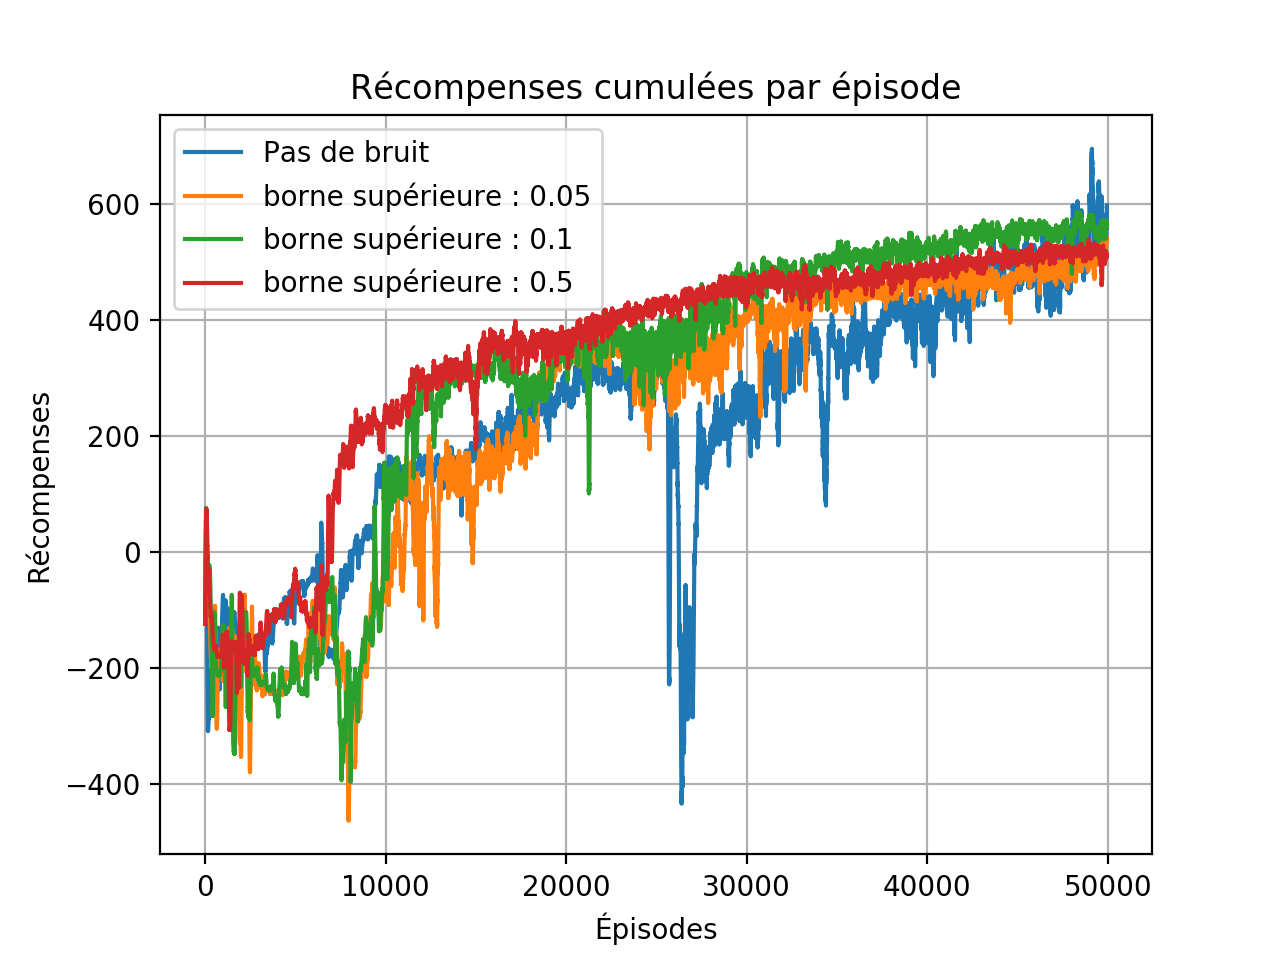
\includegraphics[scale=0.5]{assiettes/halfCheetah_uniform.png}
\caption{Influence d'un bruit uniforme centré pour le demi guépard}
\label{fig4}
\end{center}
\end{figure}
Il semblerait que mettre un léger bruit permette de réduire la variance de la récompense au cours de l'apprentissage, et d'accélérer légèrement la convergence comme montré sur la figure ~\ref{fig4}.
\smallbreak
Étudions maintenant le cas d'un processus gaussien blanc, non corrélé dans le temps (contrairement à l'article).
 
\begin{figure}
\begin{center}
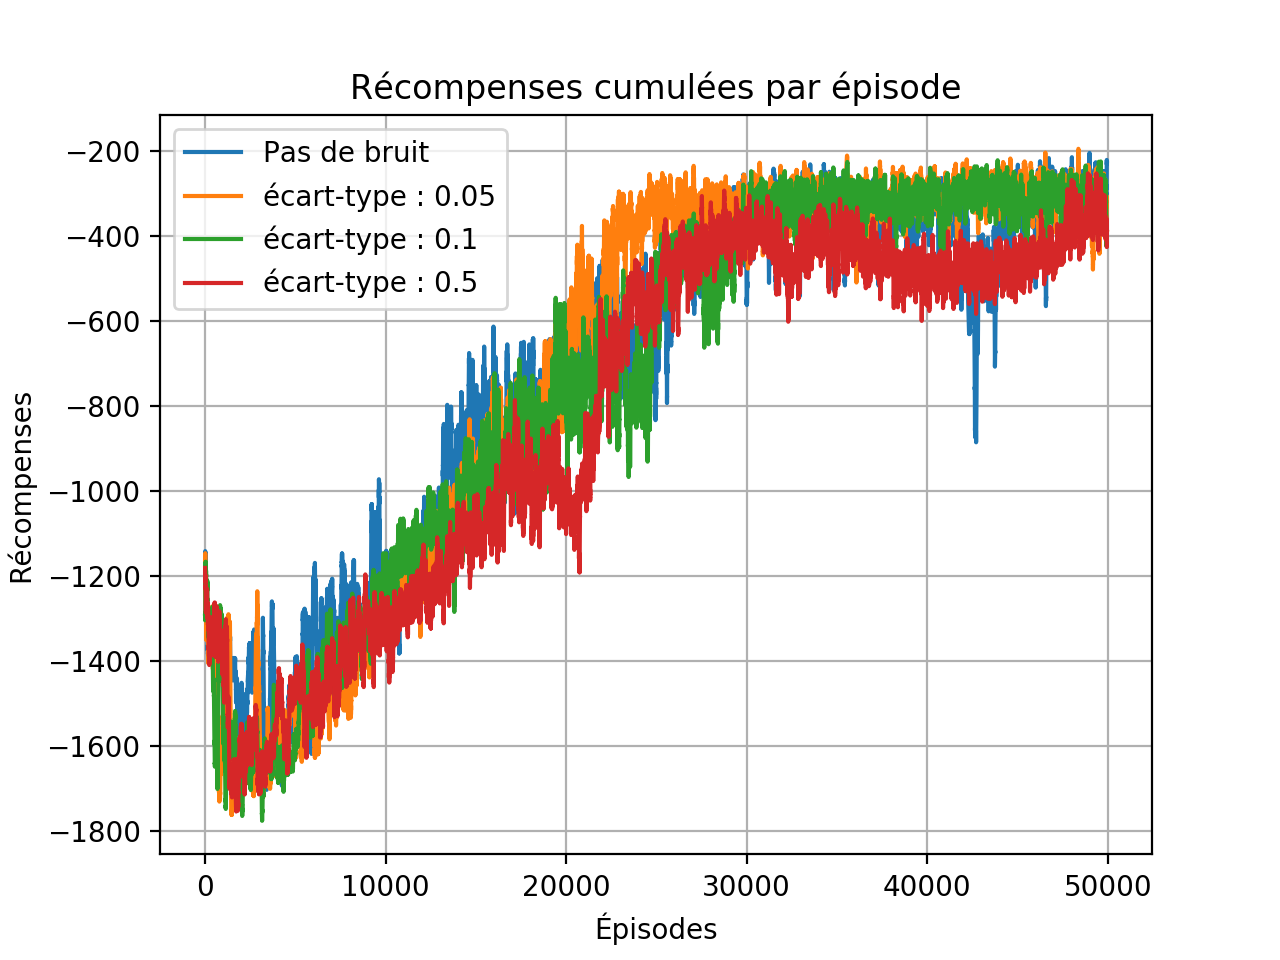
\includegraphics[scale=0.5]{assiettes/pendulum_normal.png}
\caption{Influence d'un bruit gaussien centré pour le pendule}
\label{fig5}
\end{center}
\end{figure}
Ici, sur la figure~\ref{fig5}, nous voyons que l'impact est faible. Le problème pendulum étant simple, il est possible que nous puissions converger de toute façon.

\begin{figure}
\begin{center}
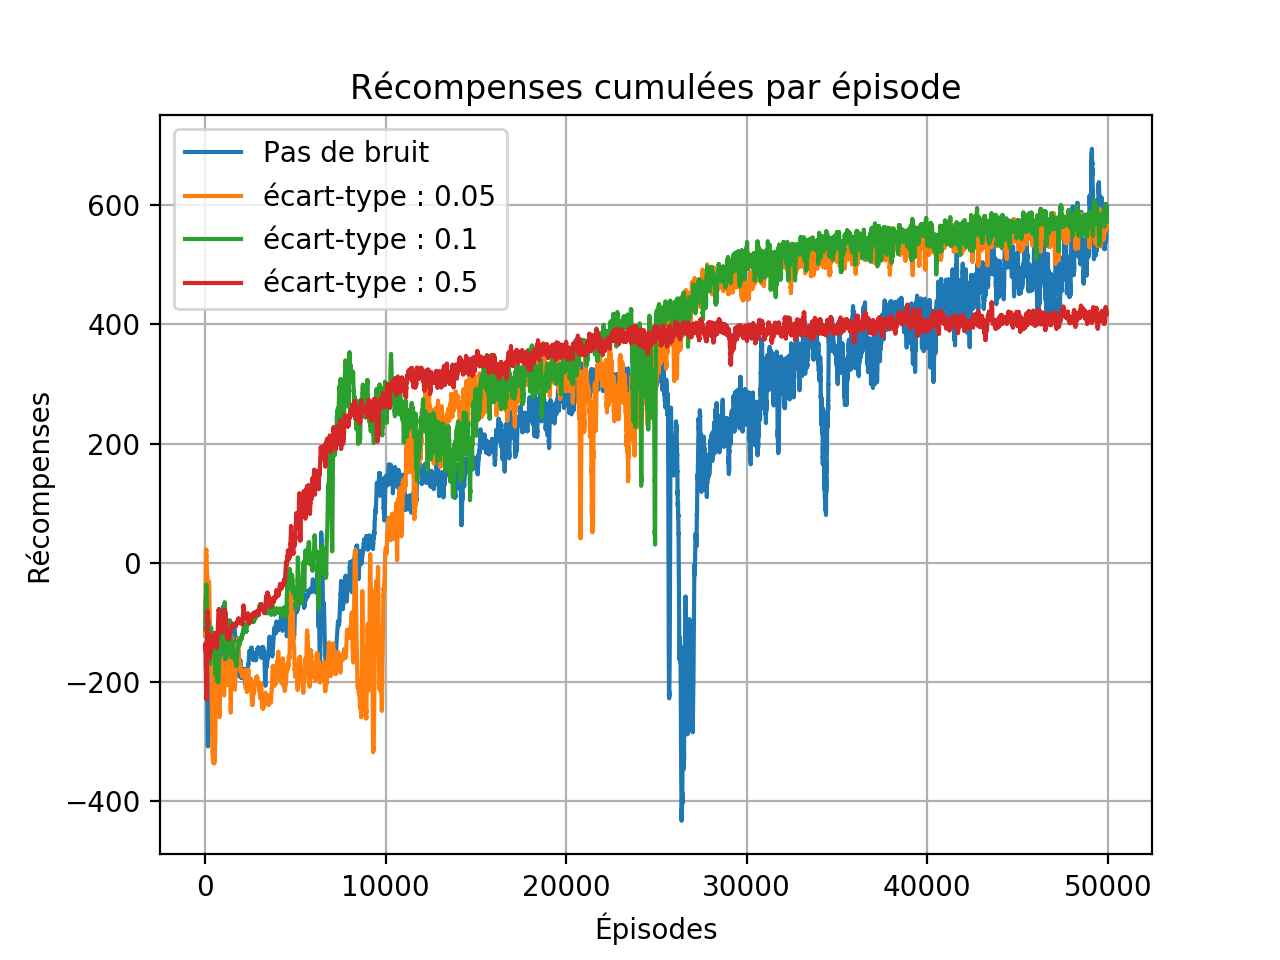
\includegraphics[scale=0.5]{assiettes/halfCheetah_normal.png}
\caption{Influence d'un bruit gaussien centré pour le demi guépard}
\label{fig6}
\end{center}
\end{figure}
Dans le cas du demi guépard, figure~\ref{fig6}, nous observons qu'un bruit trop fort abaisse le "plafond" d'apprentissage : nous restons bloqués à un score de 400, alors qu'avec une petite valeur de bruit, nous pouvons atteindre 600. Comme pour le cas uniforme, l'ajout d'un petit bruit réduit la variance de la récompense, et accélère la convergence.
\\
Jusqu'à maintenant, le type de bruit semble peu importer; l'essentiel semble être d'introduire un petit bruit dans l'exploration, accélérant ainsi la convergence (découverte de politiques novatrices facilitée).
\smallbreak
La figure~\ref{fig7} montre la performance pour les réglages de bruit correspondant au processus d'Ornstein-Uhlenbeck utilisé par les auteurs de l'article. Étonnamment, la récompense par épisode stagne à 500, ce qui est moins que ce que nous avions obtenu avec des processus gaussiens décorrélés temporellement.


\begin{figure}
\begin{center}
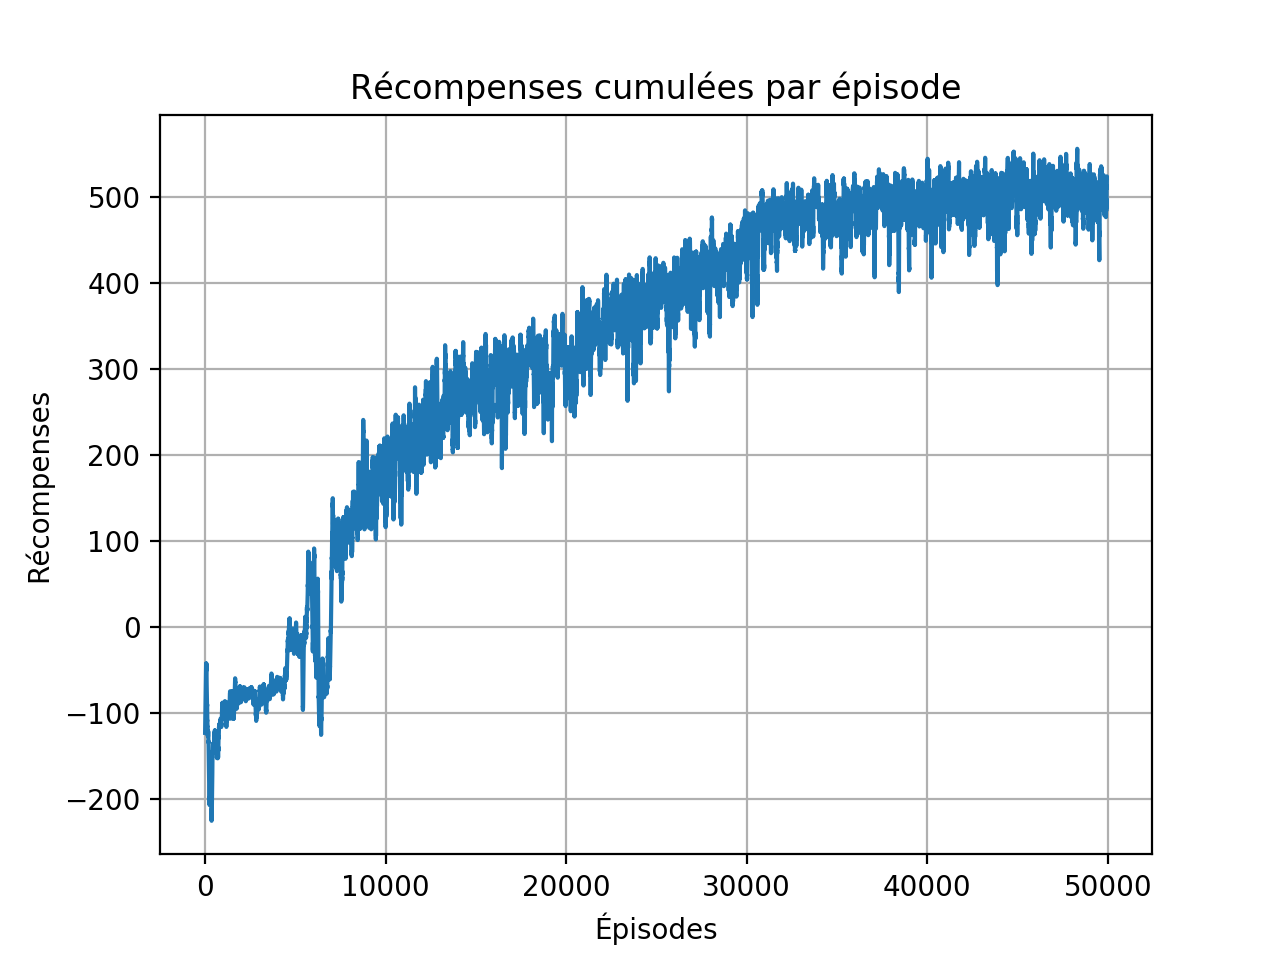
\includegraphics[scale=0.5]{assiettes/halfCheetah_ornstein-uhlenbeck.png}
\caption{Influence du bruit Ornstein-Uhlenbeck pour le demi guépard}
\label{fig7}
\end{center}
\end{figure}


\paragraph{}
La figure \ref{reseau2} montre les résultats d'expérimentations où nous avons légèrement changé le réseau du critique, en introduisant les actions au niveau de la couche d'entrée, avec les états, au lieu d'attendre la deuxième couche cachée comme ce qui était initialement présenté dans l'article. Nous observons que nous conservons, voire améliorons légèrement les propriétés de convergence de notre réseau. 

\begin{figure}
\begin{center}
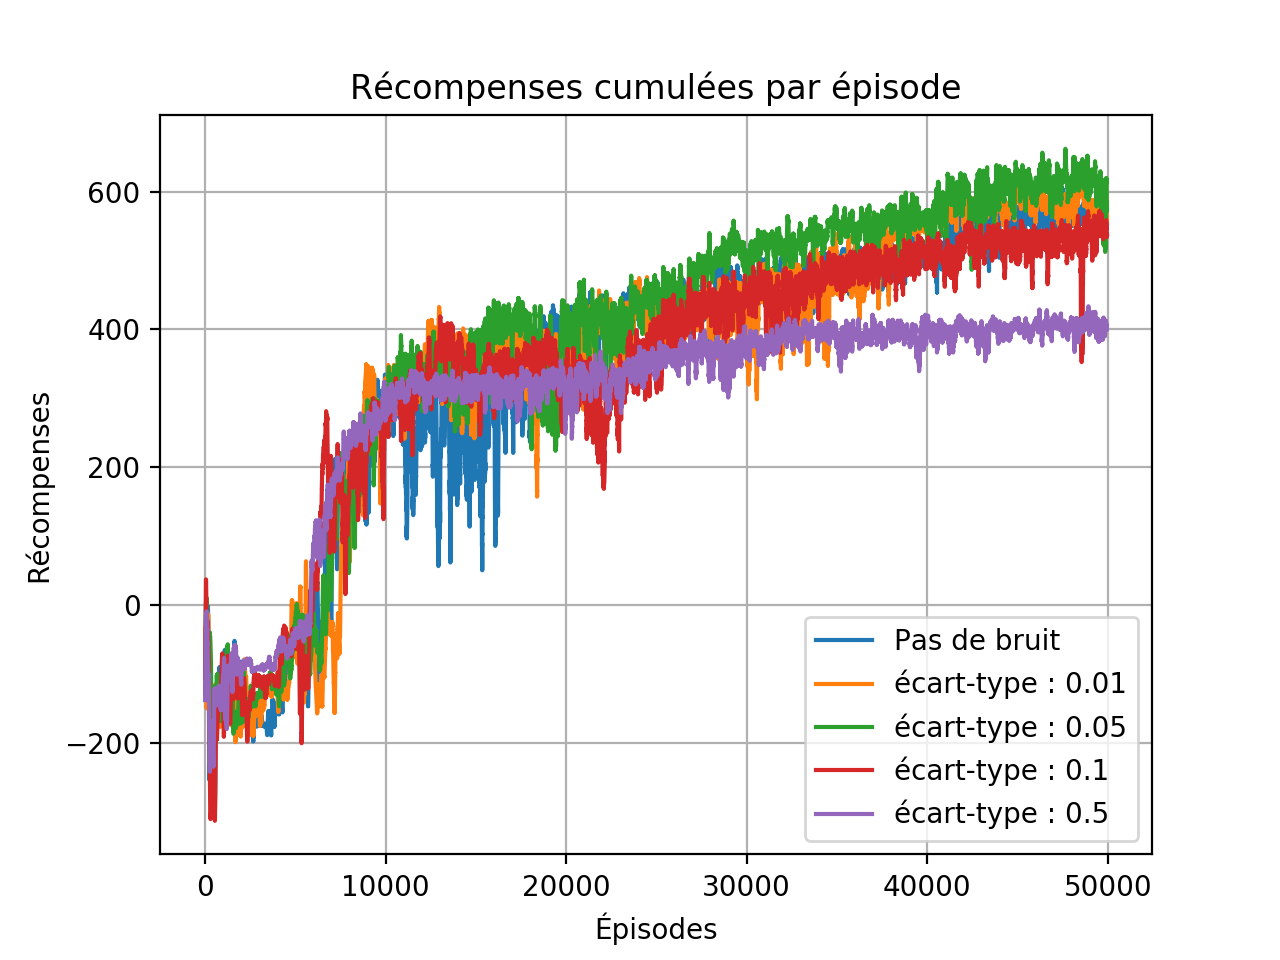
\includegraphics[scale=0.5]{assiettes/halfCheetah_uniform_action_input.png}
\caption{Influence de l'injection des actions à la première couche du réseau, pour un bruit uniforme, sur le demi guépard}
\label{reseau2}
\end{center}
\end{figure}



\section{Conclusion}
L'algorithme DDPG étudié permet l'apprentissage de politiques à plusieurs actions continues avec coordination, commme dans le cas des pattes du demi guépard. Si nous percevons l'apport positif d'un petit bruit d'exploration dans le choix des actions à évaluer, l'intérêt de décaler l'entrée des actions à la deuxième couche cachée dans le réseau critique n'a pas été démontré. La raison pour laquelle les auteurs avaient opté pour ce choix n'est pas claire; il aurait été pertinent de laisser l'algorithme se dérouler sur un plus long horizon, comme celui utilisé par les auteurs de DDPG, afin de vérifier si une différence survient plus tard au cours des expériences. Tout compte fait, notre approche aura sûrement manqué de raffinement, puisque nous n'avons pas testé sur tous les environnements proposés par les auteurs de DDPG lors de leurs propres tests, ni avec les horizons qui étaient également suggérés. Toutefois, étant donné le temps très long requis pour faire rouler ces environnements avec beaucoup de cycles, nous sommes satisfaits de l'étendue couverte par nos méthodes.

\section{Lien vers notre Github}
\url{https://github.com/JustineSurGithub/INF8225}
% References and End of Paper 
% These lines must be placed at the end of your paper 
\bibliography{Bibliography} 
\bibliographystyle{aaai} 
\end{document} 
